% \begin{frame}
%     \frametitle{Visualizzare ed Elaborare documenti XML}
%     \addtocounter{nframe}{1}
    
%     %\begin{center}
%     %    
\includegraphics[width=.2\textwidth]{../imgs/tei-r.pdf}
%     %\end{center}
%     %\textit{In parte già disponibili nei moduli TEI di base}

%      \begin{block}{Perché visualizzare il testo}
%     %     \emph{Per la critica testuale indispensabili i moduli}
%          \begin{itemize}
%             \item  Controllare la codifica e correggere i refusi
%              \item Assicurarsi che tutto sia stato trascritto correttamente
%              \item Mostrare il testo a persone che non conoscono XML-TEI
%              \item Disporre di una versione del lavoro fuibile
%         \end{itemize}
%      \end{block}
    
% \end{frame}

% \begin{frame}
%     \frametitle{Visualizzare ed Elaborare documenti XML}
%     \addtocounter{nframe}{1}
    
%     \begin{center}
%         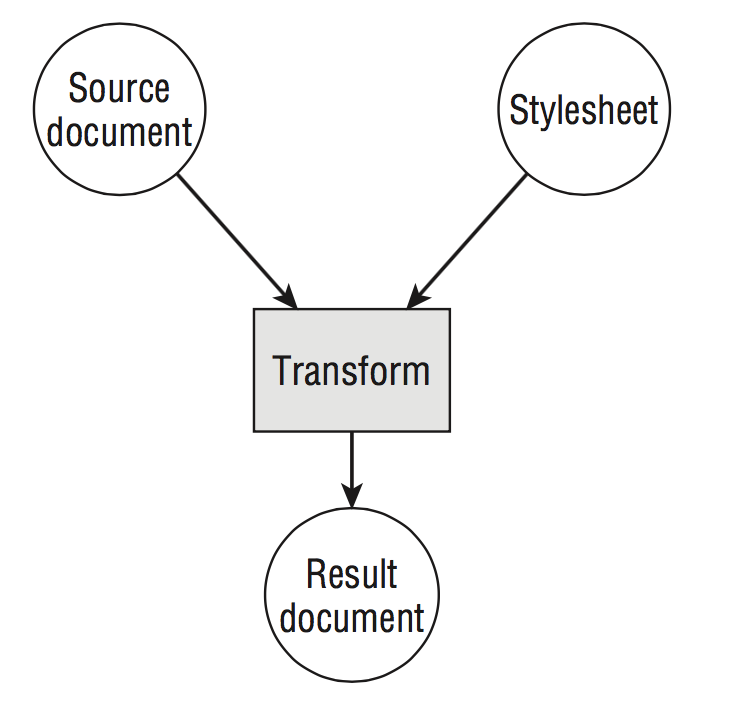
\includegraphics[width=.9\textwidth]{imgs/SchemaXSLTprocessing.png}
%     \end{center}
%     %\textit{In parte già disponibili nei moduli TEI di base}

% \end{frame}

\begin{frame}
    \frametitle{Visualizzare ed Elaborare documenti XML}
    \addtocounter{nframe}{1}
    
    %\begin{center}
    %    
\includegraphics[width=.2\textwidth]{../imgs/tei-r.pdf}
    %\end{center}
    %\textit{In parte già disponibili nei moduli TEI di base}

    \begin{block}{XPath}
        
        XPath è un \textit{expression language} fondamentale per realizzare fogli di stile XSLT.
        
    \end{block}
     
    \begin{block}{XPath}
        \begin{itemize}
            \item Selezionare nodi in un documento XML
            \item Fare match nell'albero source per selezionare il corretto template
            \item Manipolare dati attraverso funzioni
        \end{itemize}
    \end{block}
    
\end{frame}

\begin{frame}
    \frametitle{Visualizzare ed Elaborare documenti XML}
    \addtocounter{nframe}{1}
    
    %\begin{center}
    %    
\includegraphics[width=.2\textwidth]{../imgs/tei-r.pdf}
    %\end{center}
    %\textit{In parte già disponibili nei moduli TEI di base}

    \begin{block}{XPath}
        XPath offre una sintassi estesa (piuttosto verbosa) e una sintassi abbreviata.
    \end{block}

    \begin{block}{XPath}
        Le espressioni XPath permettono di selezionare con grande precisione elementi, attributi, ecc.
    \end{block}
    
\end{frame}

\begin{frame}
    \frametitle{Visualizzare ed Elaborare documenti XML}
    \addtocounter{nframe}{1}
    
    %\begin{center}
    %    
\includegraphics[width=.2\textwidth]{../imgs/tei-r.pdf}
    %\end{center}
    %\textit{In parte già disponibili nei moduli TEI di base}

    \begin{block}{Esempi XPath selezione con match}
        \emph{Selezionare \textit{documento XML} oppure tutti i nodi \texttt{<quote>}}
        \begin{itemize}
            \item \texttt{<xsl:template match="/" >}
            \item \texttt{<xsl:template match="quote" >}
        \end{itemize}
        
    \end{block}
     
    \begin{block}{Esempi XPath selezione con match}
        \emph{Per selezionare i nodi \texttt{<title>} "figli", "nipoti" o comunque discendenti di \texttt{<quote>}}
        \begin{itemize}
            \item \texttt{match="quote/title"} \textit{(discendente diretto - figlio)}
            \item \texttt{match="quote/*/title"} \textit{(discendente di secondo livello - nipote)}
            \item \texttt{match="quote//title"} \textit{(discendente a qualsiasi livello)}
        \end{itemize}     
    \end{block}
    
\end{frame}

\begin{frame}
    \frametitle{Visualizzare ed Elaborare documenti XML}
    \addtocounter{nframe}{1}
    
    %\begin{center}
    %    
\includegraphics[width=.2\textwidth]{../imgs/tei-r.pdf}
    %\end{center}
    %\textit{In parte già disponibili nei moduli TEI di base}

    \begin{block}{Esempi XPath selezione con match}
        \emph{Per selezionare i nodi \texttt{<quote>} con attributo \texttt{@type} (e valore \textit{book})}
        \begin{itemize}
            \item \texttt{match="quote[@type]"}
            \item \texttt{match="quote[@type='book']"}
        \end{itemize}
        
    \end{block}
     
    \begin{block}{Esempi XPath selezione con match}
        \emph{Per selezionare i nodi usando il carattere "jolly"}
        \begin{itemize}
            \item \texttt{match="*"}
            \item \texttt{match="*[@type]"}
            \item \texttt{match="*[@type='book']"}
        \end{itemize}
    \end{block}
    
\end{frame}


\begin{frame}
    \frametitle{Visualizzare ed Elaborare documenti XML}
    \addtocounter{nframe}{1}
    
    %\begin{center}
    %    
\includegraphics[width=.2\textwidth]{../imgs/tei-r.pdf}
    %\end{center}
    %\textit{In parte già disponibili nei moduli TEI di base}

    \begin{block}{Esempi XPath selezione con match}
        \emph{Per selezionare più di un elemento (operatore OR) oppure per selezionare un nodo con uno specifico ID}
        \begin{itemize}
            \item \texttt{match="title | author"}
            \item \texttt{match="id('stella_2007’)"}
        \end{itemize}
        
    \end{block}
    
\end{frame}

% selezione nodi con select

\begin{frame}
    \frametitle{Visualizzare ed Elaborare documenti XML}
    \addtocounter{nframe}{1}
    
    %\begin{center}
    %    
\includegraphics[width=.2\textwidth]{../imgs/tei-r.pdf}
    %\end{center}
    %\textit{In parte già disponibili nei moduli TEI di base}

    \begin{block}{XPath selezione con select}
        Il valore di questo attributo è un'espressione conforme al linguaggio XPath
    \end{block}

    \begin{block}{XPath selezione con select}
        L'attributo select può ricorrere a una sintassi più complessa rispetto a match
    \end{block}
    
\end{frame}

\begin{frame}
    \frametitle{Visualizzare ed Elaborare documenti XML}
    \addtocounter{nframe}{1}
    
    %\begin{center}
    %    
\includegraphics[width=.2\textwidth]{../imgs/tei-r.pdf}
    %\end{center}
    %\textit{In parte già disponibili nei moduli TEI di base}

    \begin{block}{L’attributo select è usato con le istruzioni XSLT}
        \begin{itemize}
            \item xsl:apply-templates
            \item xsl:value-of
            \item xsl:copy-of
            \item xsl:for-each
            \item xsl:sort
            \item xsl:variable
            \item xsl:param
        \end{itemize}
    \end{block}

\end{frame}

\begin{frame}
    \frametitle{Visualizzare ed Elaborare documenti XML}
    \addtocounter{nframe}{1}
    
    %\begin{center}
    %    
\includegraphics[width=.2\textwidth]{../imgs/tei-r.pdf}
    %\end{center}
    %\textit{In parte già disponibili nei moduli TEI di base}

    \begin{block}{XPath}
        Le espressioni XPath permettono di "navigare" l'albero del documento XML usando assi di navigazione (\textit{expression axes}).
    \end{block}

    \begin{block}{XPath}
        La selezione può essere assoluta o relativa al \textbf{nodo corrente} e si compone di tre parti: (\textbf{Assi}, \textbf{Test}, \textbf{Predicato})
    \end{block}
    
\end{frame}

\begin{frame}
    \frametitle{Visualizzare ed Elaborare documenti XML}
    \addtocounter{nframe}{1}
    
    \begin{center}
        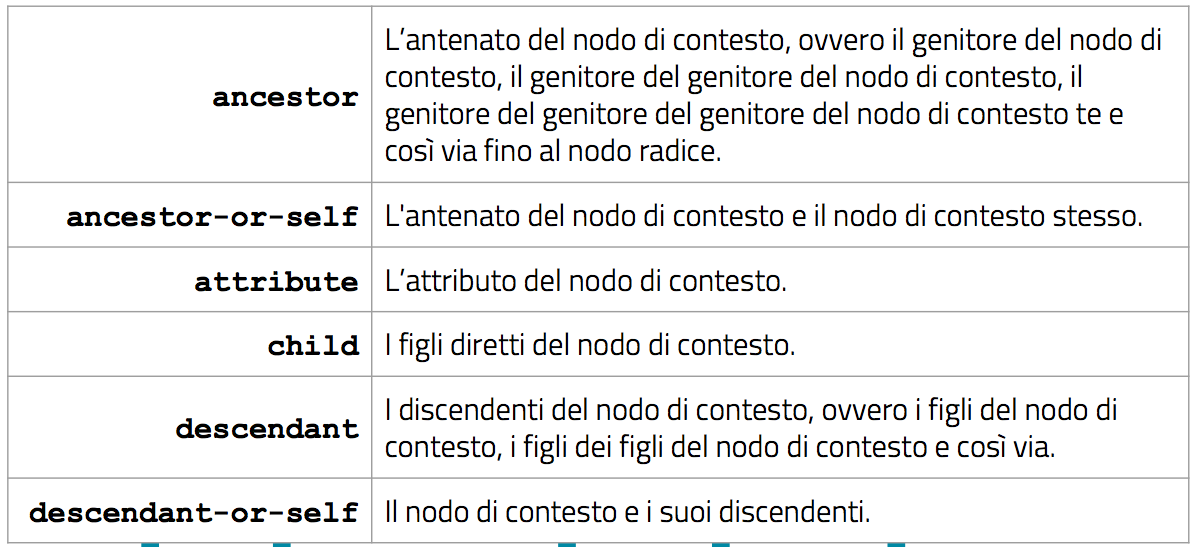
\includegraphics[width=.9\textwidth]{imgs/Schema-Assi-1.png}
    \end{center}

\end{frame}

\begin{frame}
    \frametitle{Visualizzare ed Elaborare documenti XML}
    \addtocounter{nframe}{1}
    
    \begin{center}
        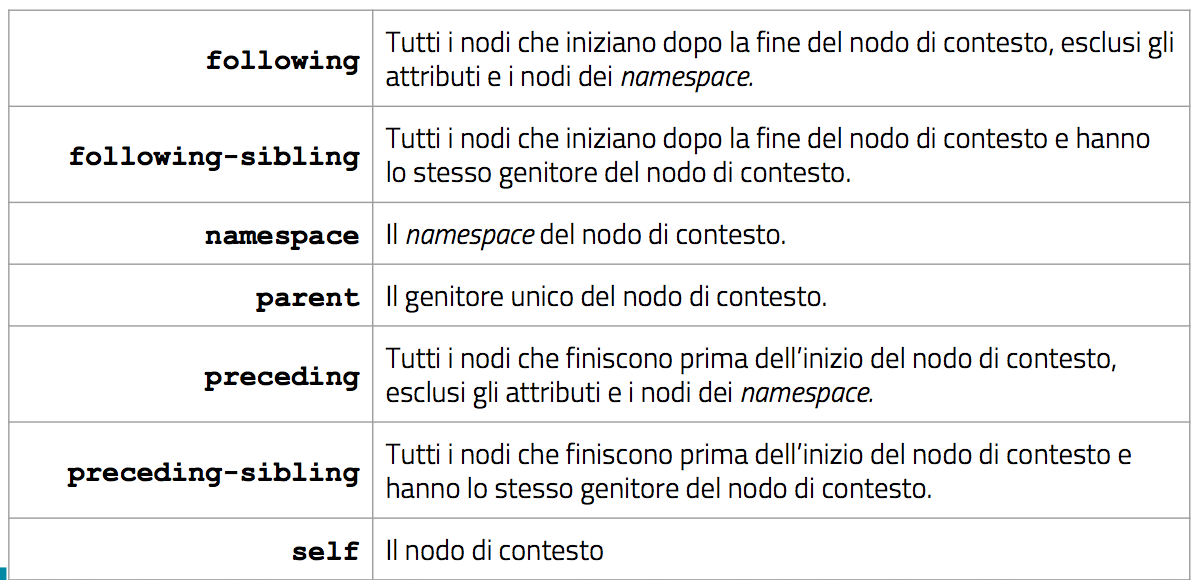
\includegraphics[width=.9\textwidth]{imgs/Schema-Assi-2.png}
    \end{center}

\end{frame}

\begin{frame}
    \frametitle{Visualizzare ed Elaborare documenti XML}
    \addtocounter{nframe}{1}
    
    \begin{center}
        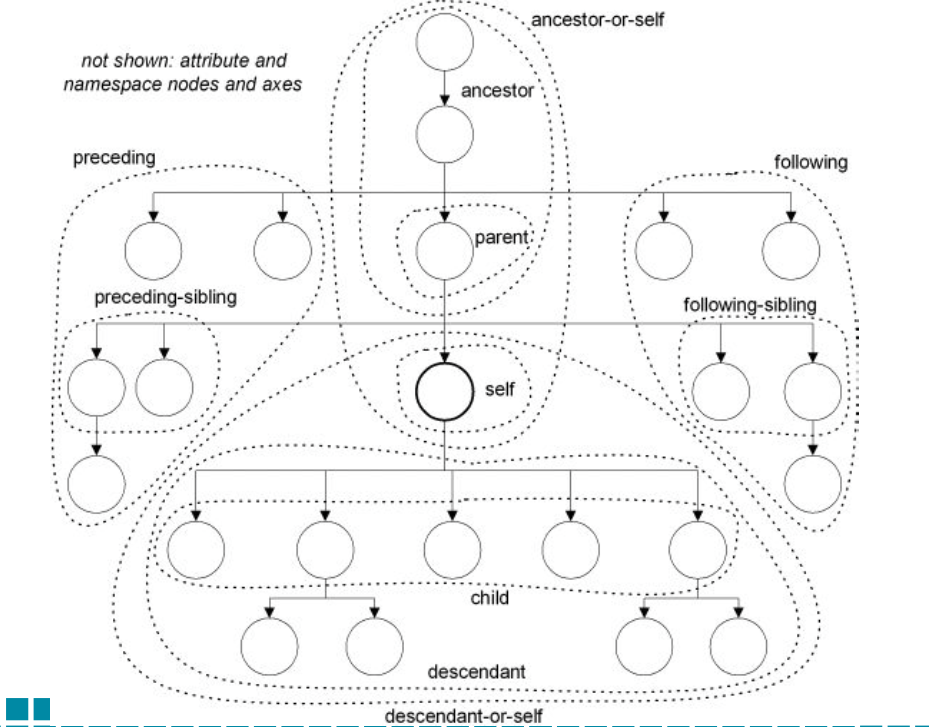
\includegraphics[width=.9\textwidth]{imgs/SchemaAssi-Xpath.png}
    \end{center}

\end{frame}

\begin{frame}
    \frametitle{Visualizzare ed Elaborare documenti XML}
    \addtocounter{nframe}{1}
    
    \begin{center}
        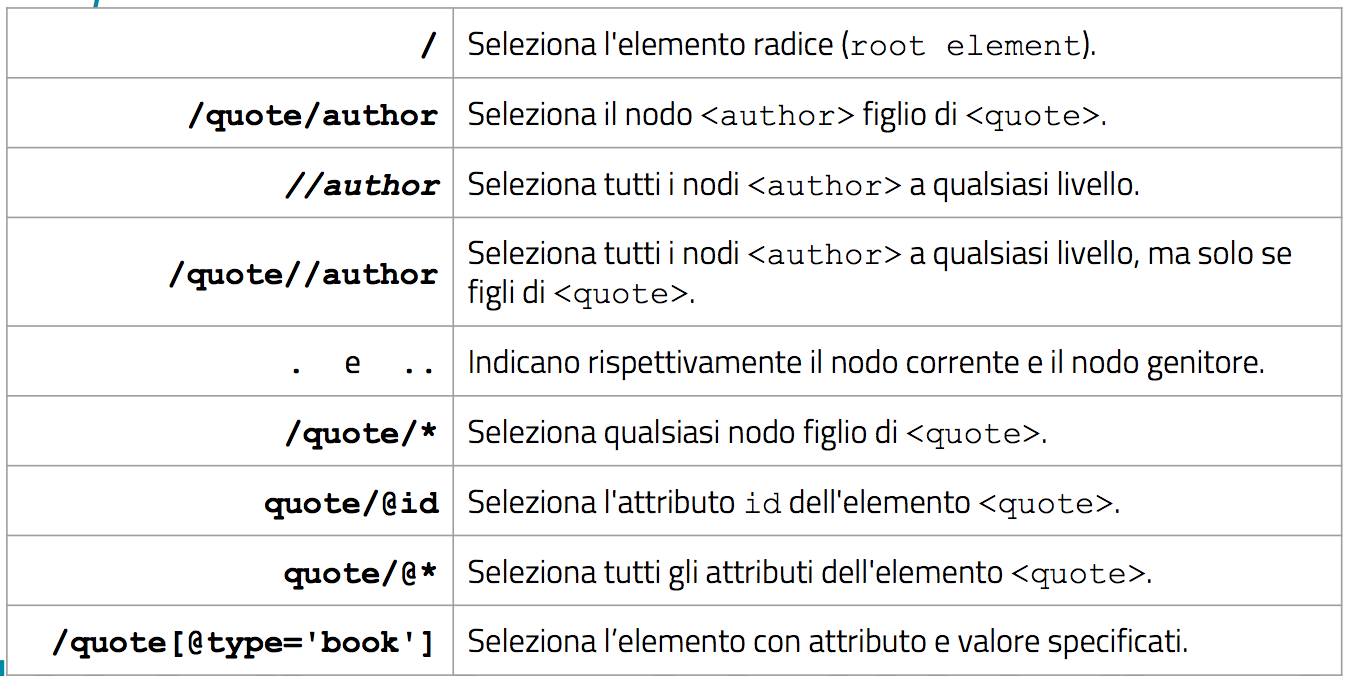
\includegraphics[width=.9\textwidth]{imgs/Sintassi-Abbreviata.png}
    \end{center}

\end{frame}


\begin{frame}
    \frametitle{Visualizzare ed Elaborare documenti XML}
    \addtocounter{nframe}{1}
    
    \begin{center}
        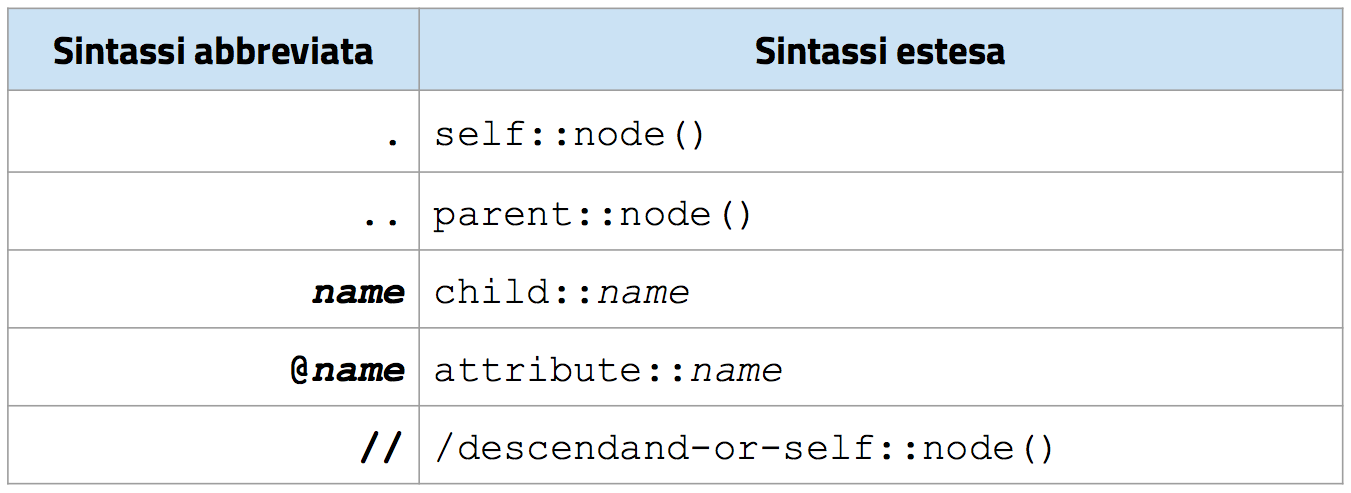
\includegraphics[width=.9\textwidth]{imgs/Sintassi-Abbreviata-Estesa.png}
    \end{center}

\end{frame}


\begin{frame}
    \frametitle{Visualizzare ed Elaborare documenti XML}
    \addtocounter{nframe}{1}
    
    \begin{center}
        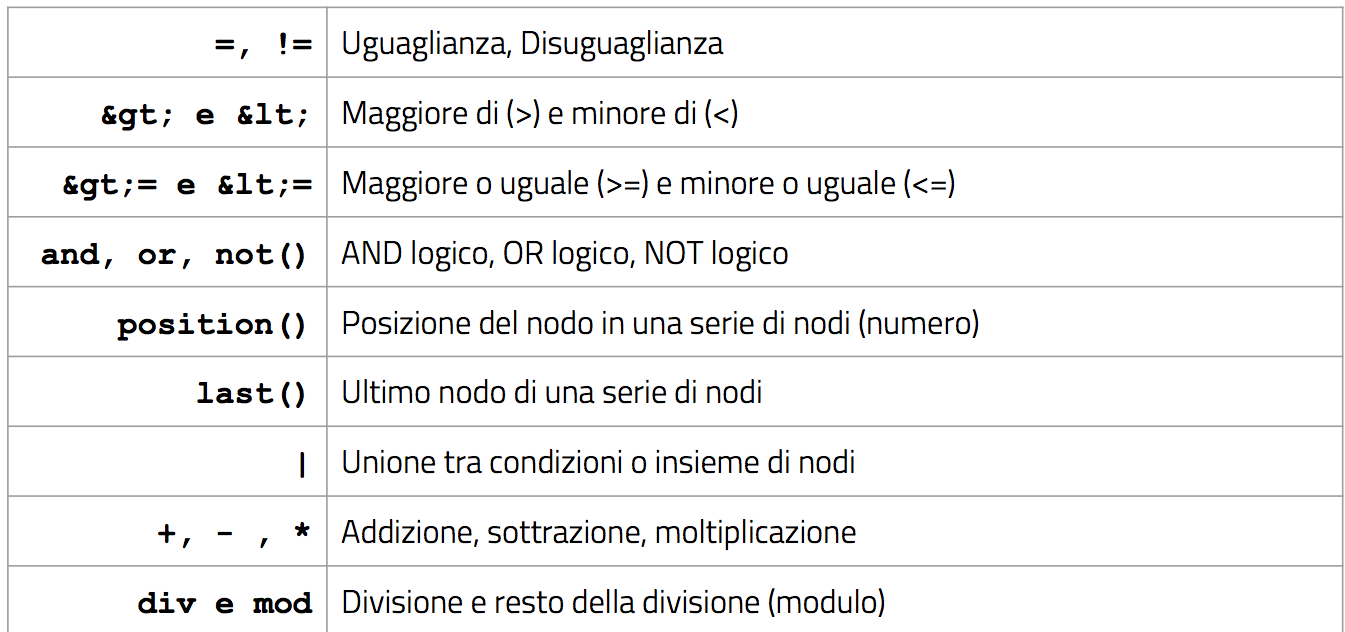
\includegraphics[width=.9\textwidth]{imgs/Tab-Operatori-Predicato.png}
    \end{center}

\end{frame}

\begin{frame}
    \frametitle{Visualizzare ed Elaborare documenti XML}
    \addtocounter{nframe}{1}
    
    %\begin{center}
    %    
\includegraphics[width=.2\textwidth]{../imgs/tei-r.pdf}
    %\end{center}
    %\textit{In parte già disponibili nei moduli TEI di base}

    \begin{block}{Esempio sintassi estesa - sintassi abbreviata}
        \begin{itemize}
            \item \texttt{<xsl:value-of select="child::author"/>}
            \item \texttt{<xsl:value-of select="author"/>}
        \end{itemize}
    \end{block}

\end{frame}

\begin{frame}
    \frametitle{Visualizzare ed Elaborare documenti XML}
    \addtocounter{nframe}{1}
    
    %\begin{center}
    %    
\includegraphics[width=.2\textwidth]{../imgs/tei-r.pdf}
    %\end{center}
    %\textit{In parte già disponibili nei moduli TEI di base}

    \begin{block}{Esempio sintassi estesa - sintassi abbreviata}
        \begin{itemize}
            \item \texttt{<xsl:value-of select="parent::quote"/>}
            \item \texttt{<xsl:value-of select="ancestor::quote"/>}
            \item \texttt{<xsl:value-of select=".."/>}
        \end{itemize}
    \end{block}

\end{frame}

\begin{frame}
    \frametitle{Visualizzare ed Elaborare documenti XML}
    \addtocounter{nframe}{1}
    
    %\begin{center}
    %    
\includegraphics[width=.2\textwidth]{../imgs/tei-r.pdf}
    %\end{center}
    %\textit{In parte già disponibili nei moduli TEI di base}

    \begin{block}{Esempio predicati}
        \begin{itemize}
            \item \texttt{//div[@type='chapter']}
            \item \texttt{//div[@type!='chapter']}
            \item \texttt{//div[@n > 2]}
            \item \texttt{//div[1]}
            \item \texttt{//div[last()]}
            \item \texttt{//div[position() = last() - 1]}
            \item \texttt{//div[position() mod 2 = 0]}
        \end{itemize}
    \end{block}

\end{frame}

